\documentclass[11pt]{article}
\usepackage{color, array, graphics}
\usepackage{amsmath}
\usepackage{amssymb}
\usepackage{enumerate}
\usepackage{mathtools}
\usepackage{fullpage}
\usepackage{graphicx}
\usepackage{float}
\usepackage{listings}
\usepackage{microtype}
\usepackage[utf8]{inputenc}

\begin{document}
\lstset{stringstyle=\ttfamily,
	showstringspaces=false,
	basicstyle=\small}

\begin{center} Alexander Garcia \hfill June 28, 2017 \\ Assignment-5 \end{center}

\medskip

\begin{enumerate}

	\item $$I = \int_{-1}^{1}e^{-2x} dx$$

	\begin{enumerate}

		\item Approximation using the composite trapezoidal rule.

		The general formula for the composite trapezoidal rule is
		\[
		I(f) = \frac{h}{2}[f(a)+f(h)+2\sum_{j=1}^{k-1}f(a+jp)]
		\]
		where $h$ is the width of the total interval, $p$ is the node width, and $k$ is the total number of nodes. In this case, $h=p = 0.5$, $k=4$, and $f = e^{-2x}$.

		Then, according to the rule,

		\[
		I(f) = \frac{0.5}{2}[f(-1) + f(1) + 2\sum_{j=1}^{3}f(a+jp)]
		\]

		or

		\[
		I(f) = \frac{1}{4}[e^{-1} + e + 2[e^{-1+0.5} + e^{-1+1} + e^{-1+1.5}]]
		\]

		When the expression is evaluated, we get the composite trapezoidal approximation of the integral to be
		\[
		I(f) \approx 2.399166\ldots
		\] \

		We know that the error for this formula can be expressed by $-\frac{h^2}{12}(b-a)f''(\eta)$, where $\eta$ is an unknown location within the interval. Rather than use an unknown location, we can bound the error by the maximum of the second derivative over the interval.

		\[f''(x) = 4e^{-2x} \leq 4e^2\ \ x\in[-1,1]\]

		Therefore, the maximum error of this approximation is
		\[
		\frac{0.5^2}{12}(1-(-1))(4e^2) \approx 1.231509\ldots
		\]

		which makes our result not very significant.

		\medskip

		\item Approximation using composite Simpson's rule

		We can define composite Simpson's rule in this case as the following
		\[
		I(f) = \frac{h}{3}\sum_{j=2}^{8}(f(a+(j-2)h) + 4f(a+(j-1)h) + f(a+jh))
		\]

		In our case, $k = 4$, and $p = \frac{b-a}{k}$, so $h = \frac{p}{2}$. We can write out the full summation then as

		\medskip

		$\frac{h}{3}$[
		\begin{tabular}{ll}
			$f(-1) + 4f(-0.75) + f(-0.5)$ & $+$ \\
			$f(-0.5) + 4f(-0.25) + f(0)$ & $+$ \\
			$f(0) + 4f(0.25) + f(0.5)$ & $+$ \\
			$f(0.5) + 4f(0.75) + f(1)$
		\end{tabular}
		]

		\medskip

		The overall error of Simpson's rule approximation can be written as

		\[
		E \leq -\frac{b-a}{180}h^4max(f''(x))\ \ x\in[-1,1]
		\]

		We can easily see that the $max(f''(x)) = 16e^2$ for our interval, so the upper bound on the error is

		We can then calculate the upper bound on the error.

		\[
		E \leq -\frac{2}{180}(0.25^4)(16e^2)
		\]
		\[
		E \leq -0.00513129\ldots
		\]

		This makes composite Simpson's approximation a much better estimate of the integral than composite trapezoidal approximation.

		\medskip

		\item For the composite trapezoidal rule, we are given that the error is defined by

		\[
		|E| \leq \frac{h^2}{12} (b-a) max(f''(x)) < 10^{-6}\ \ x\in[a,b]
		\]

		As we are simply solving for the node spacing $h$, we can rearrange this equation to gain an expression for its value.

		\[
		h  < \sqrt{\frac{12\delta}{(b-a)M}}
		\]

		where

		$M=max(f''(x))\ x\in[-1,1] = 4e^2$

		$\delta=10^{-6}$, and

		$b-a=2$.

		When these values quantities are used, we get

		\[
		h < (\sqrt{\frac{12*10^{-6}}{2*4e^2}} \approx 0.000450558\ldots)
		\] \

		\item We have a similar expression for the error of Simpson's rule

		\[
		|E| \leq \frac{b-a}{180}h^4max(f^{(iv)}(x)) < 10^{-6}\ \ x\in[a,b]
		\]

		We can again rearrange this equation to solve for $h$, the minimum node spacing to ensure an error of $\leq 10^{-6}$

		\[
		h < (\frac{180\delta}{(b-a)M})^{1/4}
		\]

		where $M=max(f^{(iv)}(x))\ \ x\in[-1,1] = 16e^2$

		$\delta = 10^{-6}$, and

		$b-a=2$.

		This inequality gives us a minimum node spacing of

		\[
		h < ((\frac{180*10^{-6}}{2*16e^2})^{1/4} \approx 0.0295381\ldots)
		\]

		\medskip

	\end{enumerate}

	\item Holmes 6.18

	\begin{enumerate}[(a)]

		\item $I_S(n) = \frac{2}{3}I_T(n) + \frac{1}{3}I_M(n/2)$

		The approximation of this integral must take place over an interval $[a,b]$, the size of which determines the node spacing $h$.
		For $n$ nodes, $h=\frac{b-a}{n}$, and for $n/2$ nodes, $h = 2\frac{b-a}{n}$. Going forward, we use these values of $h$ for $I_T(n)$ and $I_M(n)$ respectively.

		\medskip

		We know the definition of $I_M(n)$ as
		\[
		I_M(n) = h[f(a+h/2) + f(a+h) + f(a+3h/2) + f(a+2h) + \ldots + f(a+(n-1)h/2)]
		\]

		\medskip

		Considering the fact that $h=2\frac{b-a}{n}$ when we take $I_M(n/2)$, we can rewrite this equation as
		\[
		I_M(n/2) = 2\frac{b-a}{n}[f(a+2\frac{b-a}{n}) + f(a+4\frac{b-a}{n}) + \ldots]
		\]
		and
		\[
		\frac{1}{3}I_M(n/2) = \frac{2(b-a)}{3n}[f(a+2\frac{b-a}{n}) + \ldots]
		\]

		\medskip

		We also know the definition of $I_T(n)$
		\[
		I_T(n) = \frac{b-a}{2n}[f(a) + f(b) + 2f(a+\frac{b-a}{n}) + 2f(a+2\frac{b-a}{n}) + 2f(a+3\frac{b-a}{n})+\ldots]
		\]
		and
		\[
		\frac{2}{3}I_T(n) = \frac{b-a}{3n}[f(a) + f(b) + 2f(a+\frac{b-a}{n}) + 2f(a+2\frac{b-a}{n}) + \ldots]
		\]

		\medskip

		These two sequences share terms that are of the form $f(a+2i\frac{b-a}{n})$, meaning the even terms are seen twice. In $I_T(n)$, there are also multiplied by a factor of 2, meaning that in total, each even term appears 4 times. The odd terms in $I_T(n)$, then, are only found in $I_T(n)$, but are still multiplied by 2, so each odd term appears 2 times. Each end point $f(a), f(b)$ only appears in $I_T(n)$, so each has a weight of 1. When the two sequences are combined, we get
		\[
		\frac{(b-a)}{3n}[f(a) + f(b) + 4f(x_{even}) + 2f(x_{odd})]
		\]
		where $f(x_{odd}) = f(a+odd\frac{b-a}{n})$ and $f(x_{even}) = a+even\frac{b-a}{n}$. This is the definition of composite Simpson's rule.

		\medskip

		\item $I_S(n) = \frac{4}{3}I_T(n) - \frac{1}{3}I_M(n/2)$

		A very similar idea is used to demonstrate this alternate definition of composite Simpson's rule.

		\[
		\frac{1}{3}I_M(n/2) = \frac{2(b-a)}{3n}[f(a+2\frac{b-a}{n}) + \ldots]
		\]

		and

		\[
		\frac{4}{3}I_T(n) = \frac{2(b-a)}{3n}[f(a) + f(b) + 2f(a+\frac{b-a}{n}) + 2f(a+2\frac{b-a}{n}) + \ldots]
		\]

		Again, once the difference is taken, the definition of composite Simpson's rule appears.

		\[
		\frac{4}{3}I_T(n) - \frac{1}{3}I_M(n/2) = \frac{b-a}{3n}[f(a) + f(b) + 4f(x_{even}) + 2f(x_{odd})]
		\]

		\medskip

	\end{enumerate}

	\item $Q_3(f) = \frac{4h}{3}[2f(h)-f(2h)+2f(3h)]\ \ 0\leq x \leq 4h$

		\begin{enumerate}[(a)]

		\item Given that this approximation uses 3 nodes, and therefore uses three function evaluations to approximate the integral, we can say that $Q_3(f)$ is of precision $3$. This means $Q_3(f)$ can approximate integrals exactly for polynomials up to and including degree 3.

		\medskip

		\item We know that in general, the formula for the error in an odd degree Quadrature rule is
		$$E_n =  Kh^{n+1}p^n(\eta)$$
		where $h$ is the node spacing, $p^n$ is a polynomial of degree $n+1$, and $\eta$ is an unknown location on the interval. In order to find the value of $K$, we chose the function $f(x) = x^4$, where $f^{(iv)}(x) = 24$. It is known that $$\int x^4 = \frac{x^5}{5}$$ so $$\int_{0}^{4h}x^4 = \frac{(4h)^5}{5}$$

		We also know the approximation, as it was given to be
		\[
		\frac{4h}{3}[2f(h)-f(2h)+2f(3h)]
		\]

		If we expand each side as a Taylor series, we get
		\[
		F(x) = \int f(x) = F(a) + hF'(a) + \frac{h^2}{2}F''(a) + \frac{h^3}{3!}F'''(a) + \ldots
		\]
		where $a$ is given as 0. We know that $F(0)$ is zero, since $F$ is a one term polynomial. $F$ can now be rewritten in terms of $f$, as the previously unknown term $F(a)$ is now gone.

		\[
		F(x) = (x-a)f(a) + \frac{(x-a)^2}{2!}f''(a) + \frac{(x-a)^3}{3!}f'''(a) + \frac{(x-a)^4}{4!}f^{(iv)}(a)
		\]

		What we are looking for is $F(4h)$. We use the Taylor expansion of $F$ to find this value. As we know that $x-a = 4h$, we can make this substitution as well.

		\[
		F(4h) = 4hf(a) + \frac{(4h)^2}{2!}f'(a) + \frac{(4h)^3}{3!}f''(a) + \frac{(4h)^4}{4!}f^{(iv)}(a)
		\]

		Remembering that $F(a)$ was being approximated by $\frac{4h}{3}[2f(h)-f(2h)+2f(3h)]$, we can expand each $f$ term in the approximation to achieve

		\[
		F^*(h) = \frac{4h}{3}[2f(a) +
		\]
		\[
		[f(a) + 2hf'(a) + \frac{4h^2}{2!}f''(a) + \frac{8h^3}{3!}f'''(a)+\ldots] -
		\]
		\[
		2[f(a) + 3hf'(a) + \frac{9h^2}{2!}f''(a) + \frac{27h^3}{3!}f'''(a) + \ldots]] + E
		\]

		If we simply compare the $f^{(iv)}(x)$ terms in each of the Taylor expansions, we see that the term for $F$ is
		$\frac{32h^5}{5!}f^{(iv)}(a)$
		, and the term for $F^*$ is $\frac{4h}{3}[\frac{(2h)^5}{5!} - \frac{(3h)^5}{5!}]f^{(iv)}(a) = -\frac{211h^5}{5!}f^{(iv)}(a)+\ldots+E$

		When we take the difference between the actual and the approximate terms, we finally see E

		\[
		E = [\frac{32h^5}{5!}+\frac{211h^5}{5!}]f^{(iv)}(a) = \frac{241h^5}{5!}+\ldots
		\]

		or, if we want to truncate the sequence by using an unknown $a$,

		\[
		E = \frac{241h^5}{5!}f^{(iv)}(\eta)
		\]

		\medskip

	\end{enumerate}

	\item Consider the value
	\[
	A = \int_{a}^{b}f(x)dx
	\]

	\begin{enumerate}[(a)]

		\item We can let
		\[
		A^* = \int_{a}^{c}f(x)dx
		\]
		such that $A^*$ satisfies
		\[
		\frac{A^*}{A} = s
		\]
		where $0<s<1$. We must first calculate the value of $\int_{a}^{b}f(x)dx$ numerically to within a specified tolerance. In order to do this, we can use any procedure we'd like. In this case, we will use the built in MATLAB routine \texttt{integral(fun,a,b)} to calculate an ``exact'' value of the area under $f(x)$ when $a\leq x \leq b$. This gives us a final result for the denominator. We also know the ratio these integrals should reach is $s$. There is only one unknown left, in the form of $\int_{a}^{c}f(x)dx$.

		\medskip

		One way to approach solving for $c$ is to use the same method to calculate $\int_{a}^{c}f(x)dx$ as was used to calculate $\int_{a}^{b}f(x)dx$. We must iterate through the domain $[a,b]$ in order to find a value of the integral that produces the correct ratio, at which point we are done.

		\medskip

		We can start by setting $c=a$, and incrementing $c$ by a node spacing $h$, which can begin as defined by the optimal node spacing for a Simpson's rule approximation, $h = (\frac{90}{24*10^6})^(1/5)$, where $10^{-6}$ is the desired error. We then iterate through the the domain, looking for values of $c$ that satisfy the inequality $(s - error) \leq \frac{A^*}{A} \leq (s + error)$. In order to improve efficiency, when the ratio is exceeded, the iteration starts over at the most recent $c$ such that $\frac{A^*}{A} \leq s$, but with the step size cut in half.

		\medskip

		\item Seen below is the implementation of the algorithm described in part (a). In summary,
		\begin{center}
		\begin{tabular}{ll}
		$f(x)$ & is defined as $x^4$ \\
		$[a,b] = [0,1]$ & is the interval of integration \\
		$s = 0.5$ & is the desired ratio \\
		$c = 0.870551$ & is the calculated result \\
		\end{tabular}
		\end{center}

		\medskip

		As a validity check,

		$A = \int_{0}^{1}x^4dx = \frac{1}{5}$

		$A^* = \int_{0}^{0.870551}x^4dx = \frac{(0.870551)^5}{5}$

		$\frac{A^*}{A} \approx 0.50000013\ldots$ which is within the given tolerance of $10^{-5}$.

		\medskip

		\begin{center}
		Definition of $f(x)$ by \texttt{fun.m}
		\end{center}
		\lstinputlisting{fun.m}

		\medskip

		\begin{center}
		\texttt{int\_ratio.m} script to calculate c
		\end{center}
		\lstinputlisting{int_ratio.m}

		\medskip

		\begin{center}
		Output of \texttt{int\_ratio.m} script
		\end{center}
		\lstinputlisting{int_ratio.txt}

		\medskip

	\end{enumerate}

	\item

	\begin{enumerate}

		\item Differentiating discrete data is usually frowned upon due to the reliance on differences of small number to obtain the derivative. The limit definition of a derivative is $\lim_{h\to0}f'(a) = \frac{f(a+h)-f(a)}{h}$, where it is clear that smaller values of $h$ in a numerical model of this will produce a more accurate result. However, when the computation is carried out, the numbers are subject to roundoff error, and as $h\to0$, the significance of the result is lost, resulting in higher and higher error. Thus, there is a limit to how close an approximation is possible with a numerical method.

		\medskip

		\item \[D(f,h) = \frac{f(x+2h) - f(x-h)}{3h}\]

		We can approximate $f(x+2h)$ by its Taylor expansion centered at 0.
		\[
		f(x+2h) = f(x) + 2hf'(x) + \frac{4h^2}{2!}f''(x) + \frac{8h^3}{3!}f'''(x) + \frac{16h^4}{4!}f^{(iv)}(x)\ldots
		\]

		Likewise for $f(x-h)$,
		\[
		f(x-h) = f(x) - hf'(x) + \frac{h^2}{2!}f''(x) - \frac{h^3}{3}f'''(x) + \frac{h^4}{4!}f^{(iv)}(x) + \ldots
		\]

		When we take this difference $f(x)$ disappears, and we are left with
		\[
		f(x+2h) - f(x-h) = 3hf'(x) + \frac{3h^2}{2!}f''(x) + \frac{9h^3}{3!}f'''(x) + \frac{15h^4}{4!}f^{(iv)}(x) + \ldots
		\]

		Rearranging for $f'(x)$, we get
		\[
		f'(x) = \frac{1}{3h}[f(x+2h)-f(x-h)-\frac{3h^2}{2!}f''(x) + \ldots]
		\]

		Dropping the unknown terms, we get the approximation for $f'(x)$
		\[
		f'(x) \approx \frac{f(x+2h)-f(x-h)}{3h} = D(f,h)
		\]

		Alternatively, we can truncate the sequence at the $f''(x)$ term by writing
		\[
		f'(x) = \frac{f(x+2h) - f(x-h)}{3h} - \frac{3h^2}{2*3h}f''(c)
		\]

		The error, then, of the approximation is this $f''(c)$ term
		\[
		E = \frac{h}{2}f''(c) = f'(x) - \frac{f(x+2h)-f(x-h)}{3h}
		\]

		\item We can express the error of the approximation through the remainder of the Taylor expansion of the approximation. We can take the quantity $A(h)$ to be an approximation to an exact quantity $F$ using node spacing $h$. Here, we expect $A$ to be an $O(h^p)$ approximation, where $p$ represents how far out one wishes to go in the Taylor expansion.
		\[
		F = A(h) + c_1h^p + c_2h^{p+1} + c_3h^{p+2} + \ldots
		\]

		If the node spacing is cut in half, as is suggested in the problem, then we can rewrite $F$ as $F^*$ where
		\[
		F = A(\frac{h}{2}) + c_1(\frac{h}{2})^p + c_2(\frac{h}{2})^{p+1} + c_3(\frac{h}{2})^{p+2} + \ldots
		\]

		It seems that $A(\frac{h}{2})$ is again an $O(h^p)$ approximation, despite taking a shorter node spacing. However, if we compute the basic difference between the $A(h)$ approximation and $2^pA(\frac{h}{2})$ approximation, we get
		\[
		2^pF - F = (2^p-1)F= [2^pA(\frac{h}{2}) + c_1h^p + c_2\frac{h^{p+1}}{2} + \ldots] - [A(h) + c_1h^p + c_2h^{p+1} + \ldots]
		\]

		Noticing that the $c_1h^p$ terms cancel out, we now get
		\[
		F = \frac{2^pA(\frac{h}{2})-A(h)}{2^{p-1}} - \frac{c_2}{2^p}h^{p+1} + \ldots
		\]

		and since the term following the approximations is $O(h^p+1)$, we see that the new result is a better approximation, since for small $h$, $h^{p+1} < h^p$.

		\medskip

	\end{enumerate}

	\item

	\begin{enumerate}

		\item \textbf{False.} The current global error is defined as the global error of the previous step multiplied by a growth factor. At each step, the error can be defined in terms of the deviation from the previous step as the local truncation error, where the initial error is 0, as otherwise the numerical solution would not satisfy the initial value. The error at the second node is then defined by the local truncation error, which is present at every following node. This means that the local truncation errors will compound one one another, growing the global error. However, as long as the numerical solution stays within a bound, say $\epsilon$ over the interval $[a,b]$, the solution is still considered stable, despite a growing global error.

		\medskip

		\item \textbf{True.} The current global error is defined as the previous global error multiplied by some growth factor, then added to the local truncation error. No matter how small this growth factor is, the local truncation error will always be added onto it, ensuring a global error of at least the sum of all local truncation errors.

		\medskip

		\item An implicit method for numerical solution requires an approximation of $y(t_{i+1})$ to be made in order to solve for $y(t_{i+1})$. This makes implicit methods much better approximations, as they can use more information about the curve to approximate a solution than an explicit method. Explicit methods rely solely on previously calculated data points to generate $y(t_{i+1})$.

		\medskip

		\item Local truncation error, as the name implies, only looks at one step in the numerical solution to a differential equation. In this case, the numerical solution is assumed correct in step $t_i$. In order to account for this, a new solution curve, $y^*(t)$ is used, which passes through the point $t_i$. The local truncation error, then is the difference between the approximation to $y(t)$ at $t_{i+1}$ and $y^*(t)$ at $t_{i+1}$.

		The global error is taken at the end of the approximation. It is the total difference, $y(t)-w(t)$ and grows/shrinks with the differential equation. If the differential equation $f(t_i,y_i)$ is large, then the global error is amplified at $t_i$.

		\medskip

		\item A stable numerical solution to an ODE will stay within a certain boundary, say $\epsilon$, of the analytical solution. For instance, if the exact solution to $f(t,y)$ is $y(t)$, then any stable numerical solution with an initial value of $\epsilon$ of $y(0)$ will stay within $\epsilon$ of $y(t)$. In other words, the error of a stable solution is bounded over the entire interval of interest. An unstable solution has an error that grows as $t$ increases.

		\medskip

		\item \textbf{True.} Some differential equations have regions of stability and instability. If a solution begins as unstable, it can still trend towards a stable region. Once the solution is in the stable region, it will trend towards the an equilibrium solution as $t\to\infty$.

		\medskip

		\item \textbf{True.} The stability of a numerical solution is dependent on not only the ODE, but also the spacing of data points that are being used to create the solution. If the jump between any two data points is too distant, then the numerical solution will not accurately represent the ODE, and could potentially vary to the point of insignificance.

		\medskip

		\item Accuracy is the primary factor in determining step size for the backward Euler method. If we let $e_i$ represent the error at a point $i$, then we can say that $e_i$ must be less than a given tolerance $\delta$, which is the maximum error over each interval. If $e_i > \delta$, then we know that the step size is too large, and therefore must shrink by some factor $q$.

		Additionally, it is known that due to its implicit nature, the backward Euler method is absolutely, unconditionally stable, and therefore the trend of the solution does not depend on the step size.

		\medskip

		\item A stiff ODE is one in which different terms dominate depending on time. For instance, a solution $y=e^{-t} + 100t$ is dominated by $100y$ for small values of $t$, as the exponential is still very small. However, as $t$ grows, $e^{-t}$ quickly overtakes the linear term, and becomes the defining feature of the equation.

		This kind of problem is difficult to solve numerically because of the changes in behavior of the solution. At one time, the slope is incredibly steep, and an numerical method requires a very tight node spacing to accurately capture this fact. However, after the exponential term begins to dominate, the solution is much easier to approximate, and much fewer nodes are required. However, because of the behavior at the beginning, a basic numerical method will still use a spacing $h$ to solve, as this is what is required at the start, which can be a very expensive procedure.

		\medskip

		\item The Taylor methods for solving an ODE numerically have a much harder time computing high order approximations. This is because the Taylor approximation uses additional derivative evaluations for every increase in order ($O(h^p)\to O(h^{p+1})$) requires one additional derivative evaluation). This can become very expensive, as each derivative is more difficult to compute than the last.

		\medskip

	\end{enumerate}

	\item % Question 7

	\begin{enumerate}

		\item % Part a

		\begin{enumerate}

			\item A stable solution of an ODE will stay within a certain bound of the exact solution over the entire interval of interest, while an unstable solution will vary greatly from point to point. In a more formal sense, a stable solution $y_1(t)$ satisfies
			\[
			|y(t)-y_1(t)| \leq \epsilon\ \ t > 0
			\]

			Even if a solution begins as unstable, it is still possible for it to become stable over time. If equilibrium solutions to the ODE exist, and one of these is stable, then there is a region, although initially unstable, that will still trend towards the equilibrium solution over time.

			\medskip

			\item

			\begin{itemize}

				\item $f=2y+t$ has stable solutions. Since $f_y > 0$ for all $y$, all solutions are stable, no matter the initial value. However, as there is no equilibrium condition, the solutions do not approach a specific value, preventing them from being asymptotically stable.

				\medskip

				\item $f=2y-t$ again has stable solutions. $f_y$ does not depend at all on the sign of $t$, so solutions will behave the same way as in the previous question.

				\medskip

				\item $f=t-2y$ has unstable solutions. Because $f_y<0$ for all $y$, all solutions are unstable, no matter the initial value. The lack of an equilibrium solution again prevents the problem from being asymptotically stable.

				\medskip

				\item $f=\frac{t}{2}$ has asymptotically stable solutions. Because the slopes of $y$ are defined explicitly (without $y$), we can exactly calculate $y$ numerically. Since a solution is asymptotically stable if $\lim_{t\to\infty}|y-y*| = 0$, and the numerical solution can be exact, then the solutions are all asymptotically stable.

				\medskip

			\end{itemize}

		\end{enumerate}

		\item $y' = -200ty^2,\ y(0) = 1$

		\begin{enumerate}

			\item Euler's method defines the next point in a sequence to be

			\[
			w_{i+1} = w_i + hf(t_i,w_i),\ w_0 = \alpha
			\]

			In this case, $\alpha = 1$, and we will use a step size $h=0.025$.

			\medskip

			\begin{tabular}{llll}

			$w_1$ & $= w_0 + hf(t_0,w_0)$ & $= 1 + 0.025[-200*0*1^2)]$ &$=1$ \\
			$w_2$ & $= w_1 + hf(t_1,w_1)$ & $= 1 + 0.025[-200 * 0.025 + 1^2]$ & $=0.875$ \\
			$w_3$ & $= w_2 + hf(t_2,w_2)$ & $= 0.875 + 0.025[-200 * 0.05 + 0.875^2]$ & $=0.683594$ \\
			$w_4$ & $= w_3 + hf(t_3,w_3)$ & $= 0.644 + 0.025[-200*0.075 + 0.644^2]$ & $=0.508356$ \\

			\end{tabular}

			\[y(0.1) \approx 0.508356\]

			\medskip

			\item An order 2 Taylor method defines the next point in a sequence to be

			\[
			w_{i+1} = s_i + hf_i + \frac{h^2}{2}f'_i,\ w_0 = \alpha
			\]

			In this case, $\alpha = 1$, and we will use a step size $h=0.025$. Additionally, since $f'_i$ is not technically known, we must represent it by
			\[
			f'_i = f_t + ff_y
			\]

			In this case,
			\[f_t = -200y^2\]
			\[ff_y = -200t * -200ty^2 = 40000t^2y^2\]

			\medskip

			\begin{tabular}{lll}

			$w_1$ & $= w_0 + hf(t_0,w_0) + \frac{h^2}{2}(f_t+ff_y)$ & $= 0.9375$ \\
			$w_2$ & $= w_1 + hf(t_1,w_1) + \frac{h^2}{2}(f_t+ff_y)$ & $= 0.779572$ \\
			$w_3$ & $= w_2 + hf(t_2,w_2) + \frac{h^2}{2}(f_t+ff_y)$ & $= 0.608647$ \\
			$w_4$ & $= w_3 + hf(t_3,w_3) + \frac{h^2}{2}(f_t+ff_y)$ & $= 0.427622$

			\end{tabular}

			\[y(0.1) \approx 0.427622\]

			\medskip

		\end{enumerate}

	\end{enumerate}

	\item The solutions to this system of differential equations was carried out by a MATLAB script \texttt{ode\_sys.m}. The script uses a simple RK2 algorithm to compute the value of each solution at 3000 time steps, plus the initial conditions. The results of the calculations are then plotted first as a solution against t, then as the solutions against one another.

	\begin{center}
	\texttt{ode\_sys.m} script. Only change in this script between parts (a) and (b) is the value of \texttt{b}, which was initially $2$ when run for part (a).
	\lstinputlisting{ode_sys.m}
	\end{center}

	\medskip

	\begin{enumerate}

		\item When the simulation is done with $\beta = 2$, the two masses seem to be within ``critical'' ratios of one another. They both oscillate over time, never decaying in amplitude. When graphed against each other, they form an almost circular pattern, not converging to anything in particular.

		\begin{figure}[H]
		\centering
		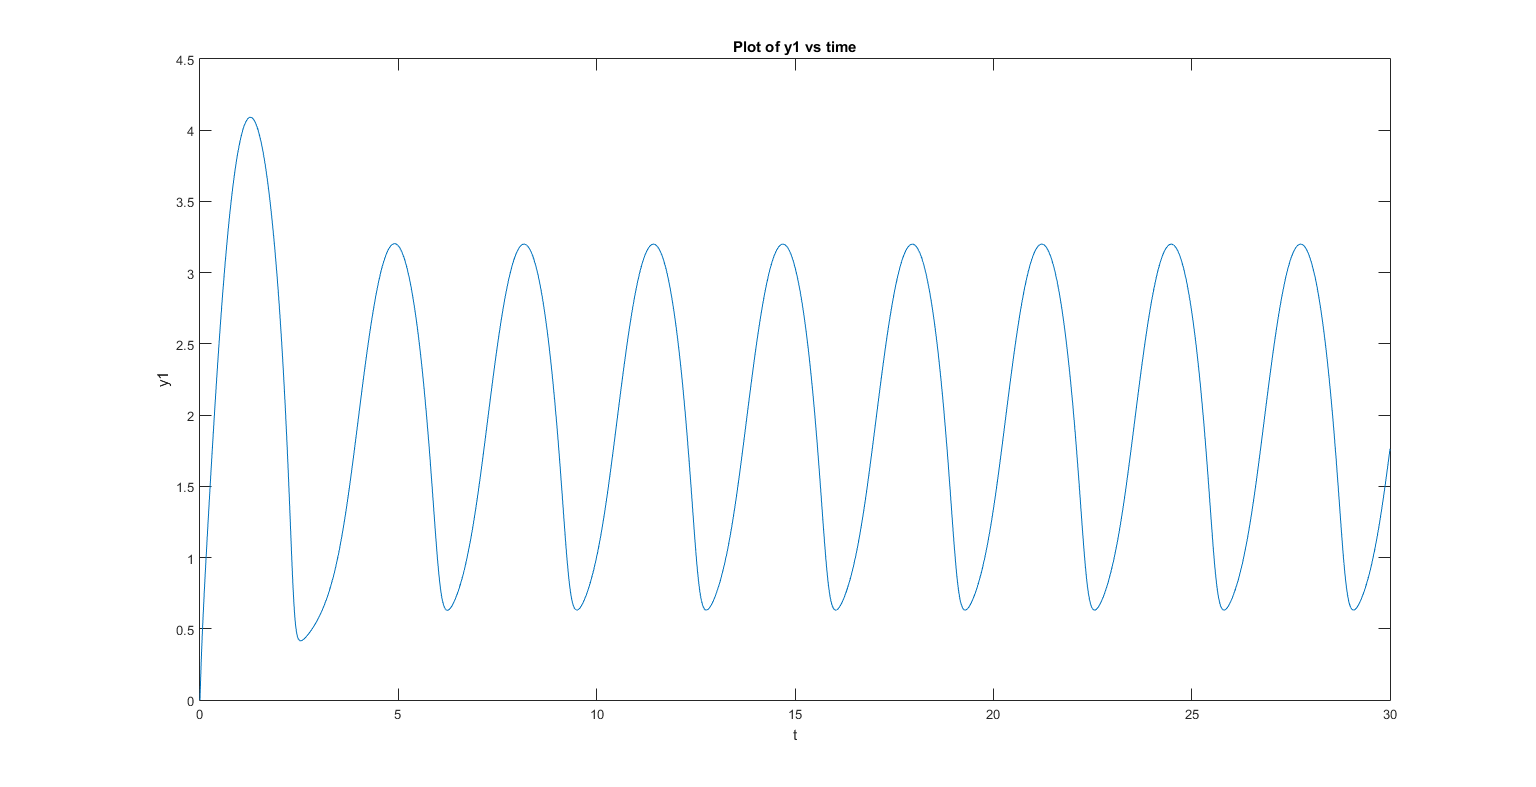
\includegraphics[width=\textwidth]{8a1.png}
		\end{figure}

		\medskip

		\begin{figure}[H]
		\centering
		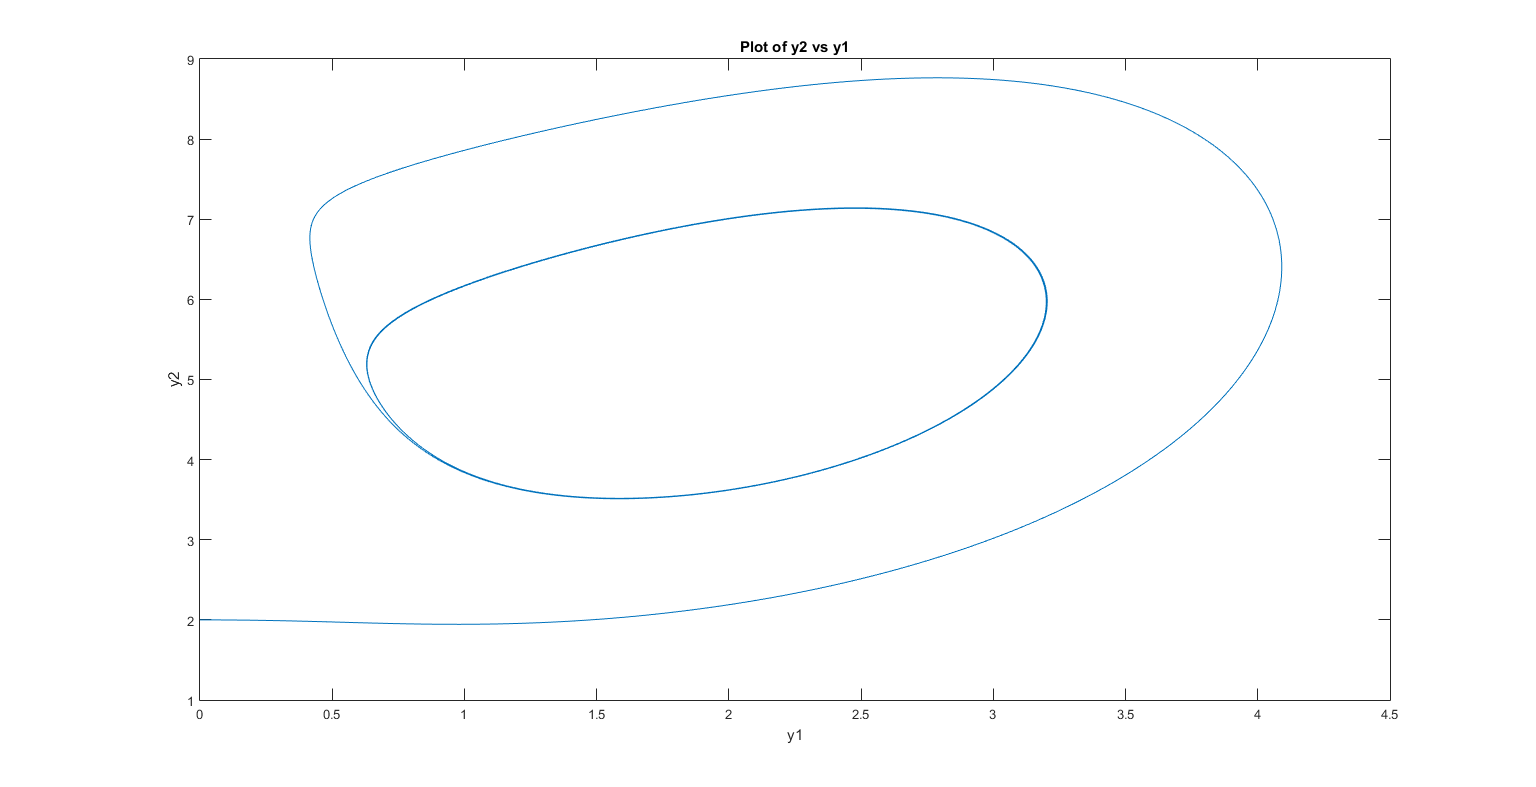
\includegraphics[width=\textwidth]{8a3.png}
		\end{figure}

		\medskip

		\item When the simulation is done with $\beta=4$, however, the two masses seem to converge, with $y_1 \to 2$ and $y_2 \to 5$. Clearly the $\beta$ factor in front of $y_2'(t)$ has a large impact on the convergence of solutions for this system.

		\begin{figure}[H]
		\centering
		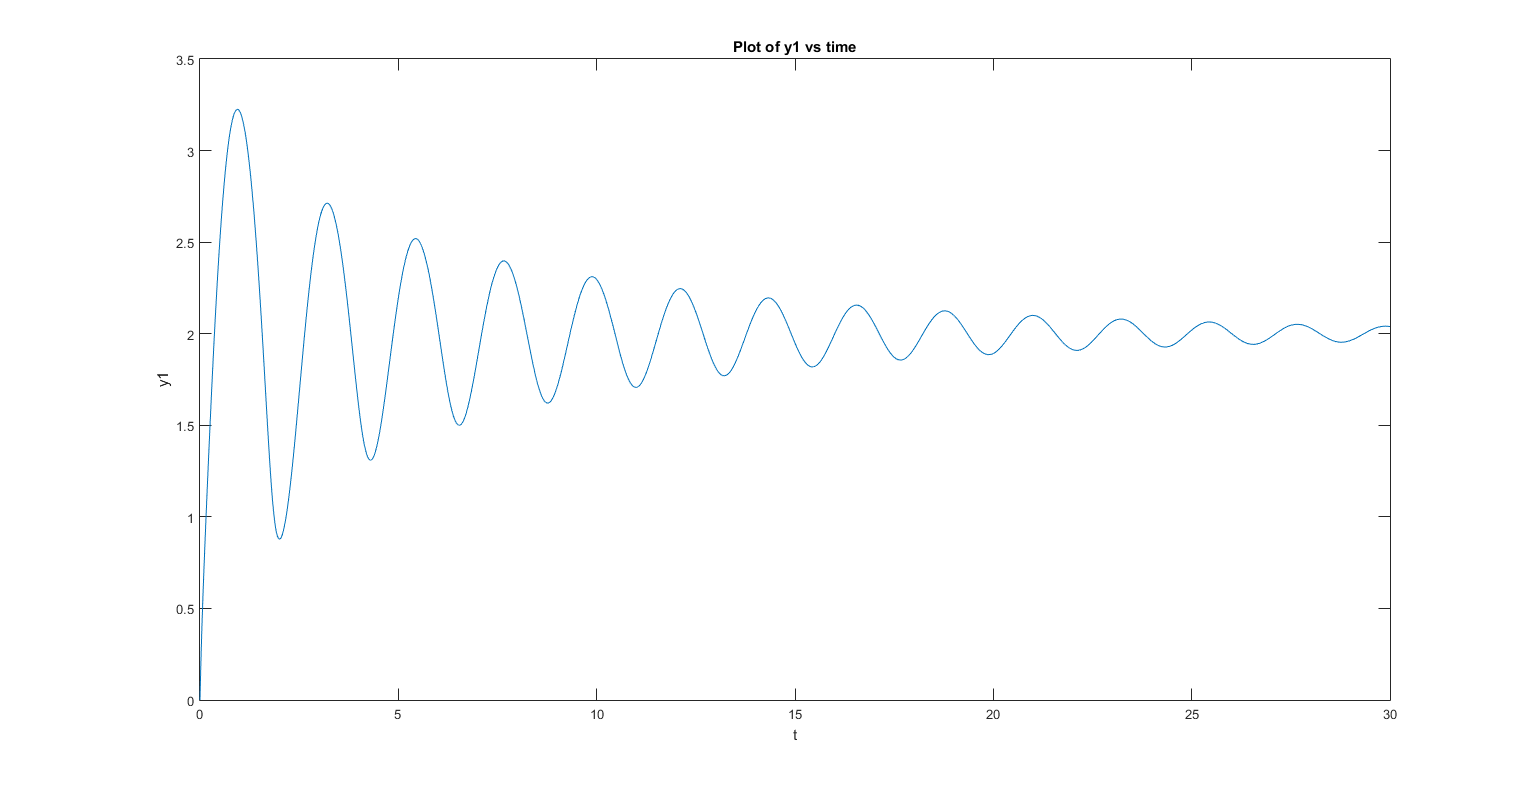
\includegraphics[width=\textwidth]{8b1.png}
		\end{figure}

		\medskip

		\begin{figure}[H]
		\centering
		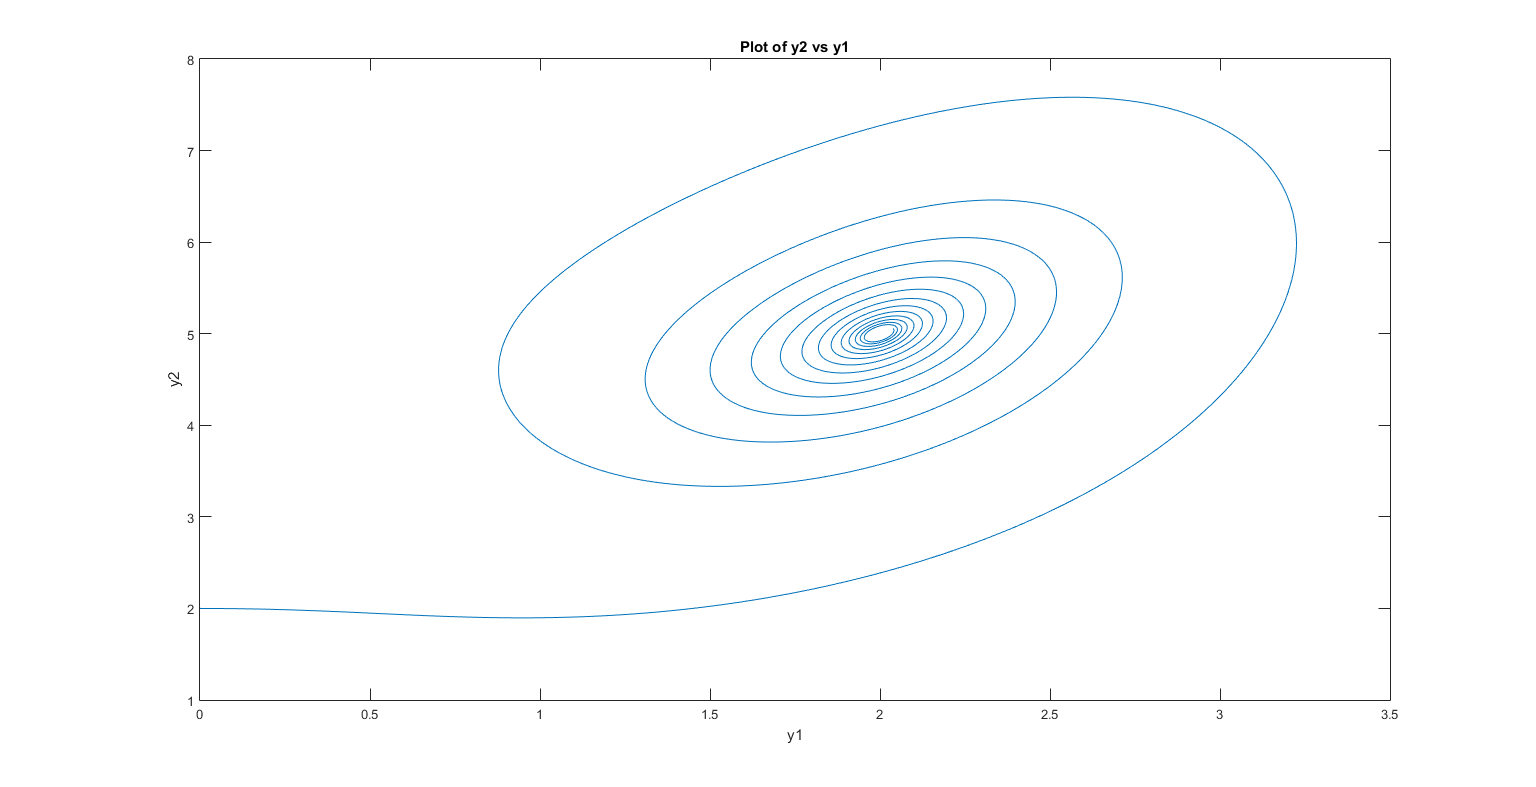
\includegraphics[width=\textwidth]{8b3.png}
		\end{figure}

	\end{enumerate}

\end{enumerate}

\end{document}
